\chapter{ShareTrace Implementation Notes}

\par Prior to my work on ShareTrace, I had no experience developing an algorithm that (at least hypothetically) required scalability. Ultimately, I implemented five designs of risk propagation, each providing insight that allowed for iterative improvement in performance. The following provides motivation and context for each design, along with rationale for pursuing an alternative approach.

\section{Thinking Like a Vertex}\label{sec:giraph}

% TODO Add repo citation after code cleanup
% TODO Where to specify contact search?
% TODO Cite TLAV
\par The first iteration of risk propagation utilized Apache Giraph \cite{Giraph2020}, an open-source version of the iterative graph-processing library, Pregel \cite{Malewicz2010}, which is based on the bulk synchronous parallel model for distributed computing \cite{Valiant1990}. Giraph follows the think-like-a-vertex paradiagm for graph-processing algorithms in which the algorithm is specified from the perspective of a vertex. As a highly scalable framework for graph-based algorithms, Giraph was a natural choice for implementing risk propagation. Figure \ref{fig:v1-architecture} describes the full compute architecture. 

\begin{figure}[htbp]
	\centering
	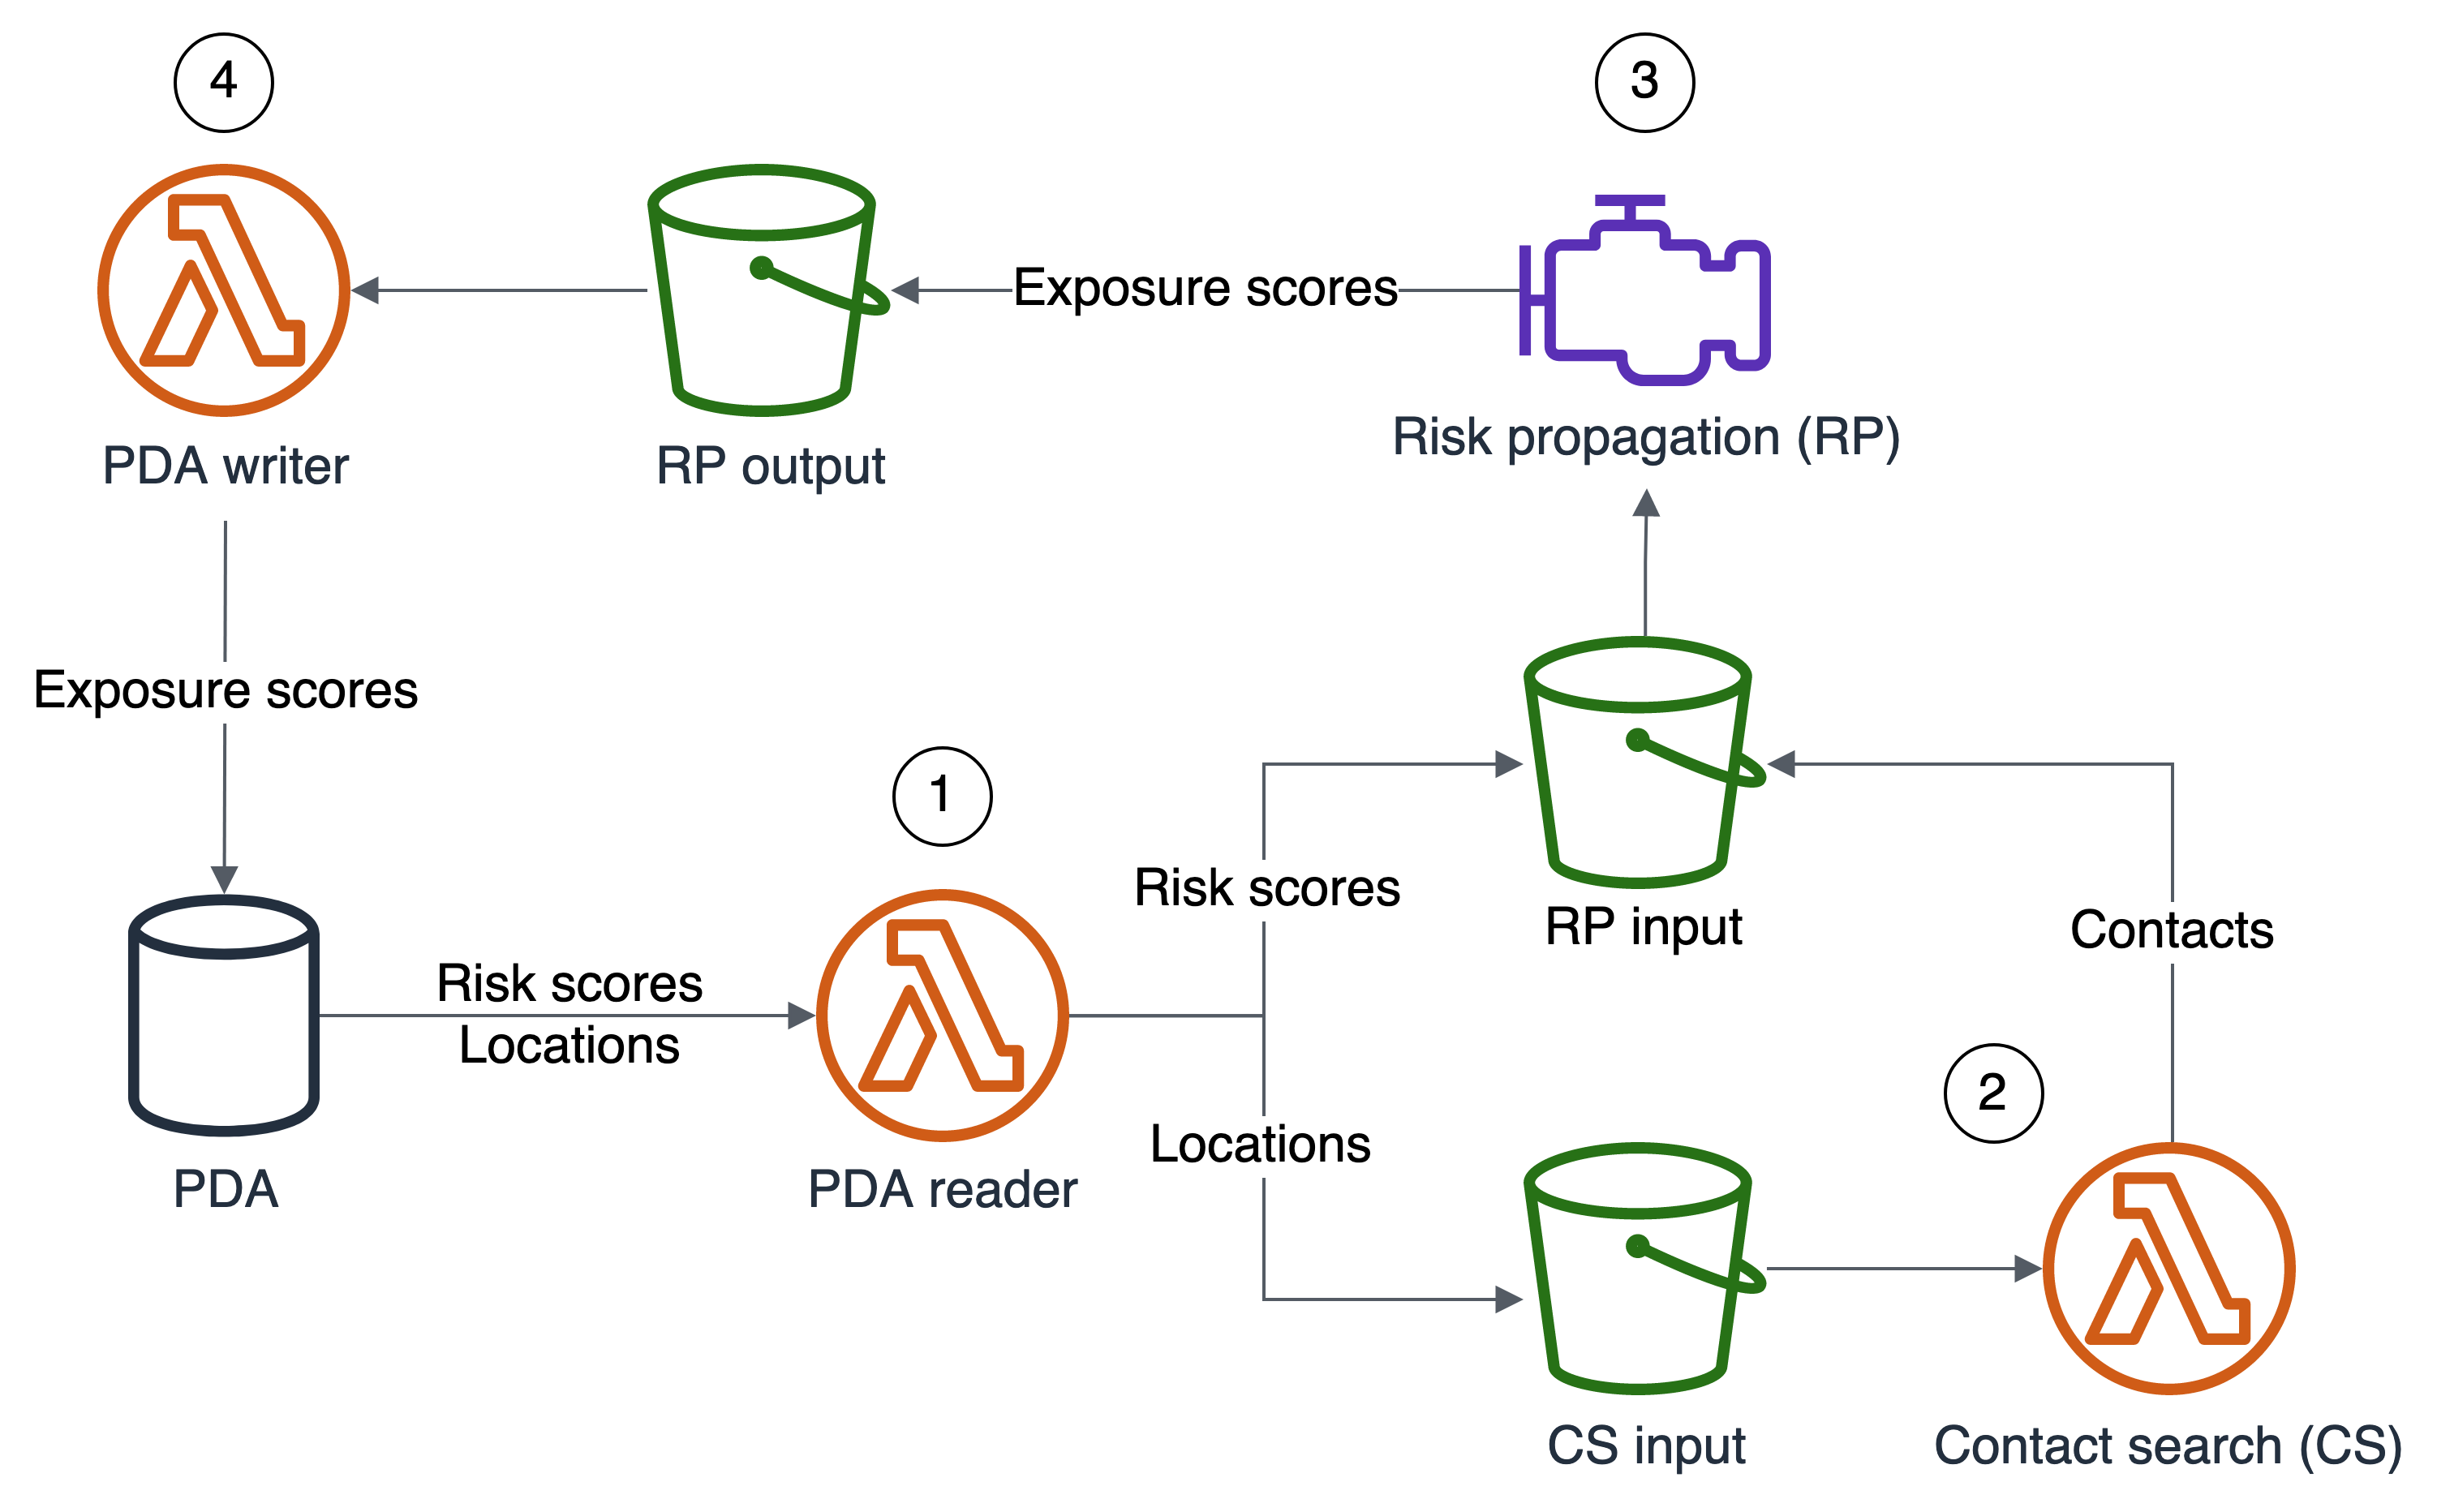
\includegraphics[width=\textwidth]{v1-architecture}
	\caption[ShareTrace batch-processing architecture]{ShareShareTrace batch-processing architecture. 
		(1) An AWS Lambda function retrieves the risk scores (symptom scores and previously computed exposure scores) and location histories from all user PDAs. Risk scores are transformed into vertex inputs for risk propagation and stored in an Amazon Simple Service (S3) bucket. Location histories are stored in a separate S3 bucket for contact extraction. (2) An AWS Lambda function executes contact search on the location histories to find all contacts, maps them to edge inputs for risk propagation, and stores them in the same S3 bucket that holds the vertex inputs. (3) Amazon Elastic MapReduce (EMR) runs risk propagation as a batch job and outputs the computed exposure scores into an S3 bucket. (4) An AWS Lambda function writes the exposure scores to the PDA of their respective user.}
	\label{fig:v1-architecture}
\end{figure}

% TODO Cite AWS Batch, S3, EMR, Lambda, Step Function
% TODO Cite fan-out pattern
\par The functionality implemented by all AWS Lambda functions was intended to follow a fan-out design in which one Lambda function would be invoked and then distribute the work amongst one or more other Lambda functions. For example, the PDA reader Lambda function would retrieve the list of all HATs and then partition that list among several other Lambda functions to retrieve user data in parallel.

\par The Giraph-based implementation is a literal interpretation of the original ShareTrace algorithm \cite{Ayday2021}. That is, it assumes a factor graph in which a factor vertex contains the contact times between two users and a variable vertex contains the maximum risk score it has received from a neighboring factor vertex. The algorithm haults when either a given number of iterations has elapsed or the total change in variable vertex values drops below a given threshold.

\par Several factors prompted the search for an alternative design to Giraph:

\begin{enumerate}
	\item \emph{Design complexity}. For a relatively straightforward data flow, the architecture in Figure \ref{fig:v1-architecture} corresponds to over 4,000 lines of source code. In retrospect, a more suitable approach than manually configured Lambda  functions would have been a managed batch-processing or workflow orchestration service, such as AWS Batch or AWS Step Function. Additionally, the low-level design of the Giraph implementation was unnecessarily complex. One-mode projection that is used in Sections \ref{sec:projected-subgraphs} and \ref{sec:vertex-actors} would have avoided the complexity of multiple vertex types. Regardless, the implementation was overengineered.
	\item \emph{Dependency management incompatability}. A major cause for redesigning the implementation was the dependency version conflicts between Giraph and the libraries used for the ShareTrace implementation. In spite of the several attempts (e.g., using different library versions, using different versions of Giraph, and forcing specific transitive dependency versions) to resolve these conflicts, a lack of personal development experience and stalled progress prompted me pursue alternatives to Giraph.
	\item \emph{Persistent data storage external to the PDA}. One of the core tenets of Dataswift is that the user fully controls the access to their data. However, as shown in Figure \ref{fig:v1-architecture}, user data is stored in S3 buckets. While it is possible to encrypt S3 objects at rest and automatically delete objects after a certain duration, data persistence to any extent is neither ideal nor desired for a privacy-preserving contact tracing solution.
\end{enumerate}

% TODO Cite Plasma object store
% TODO Cite GitHub repo after code clean up
\section{Subgraph Actors}\label{sec:subgraph-actors}

\par Attempting to mimic the design in Section \ref{sec:giraph}, I implemented risk propagation using the Python library, Ray  \cite{ray2021} that ``provides a simple, universal API for building distributed applications.'' While it claims to support actor-based programming, Ray provides relatively basic support compared to Akka, which is used in the current implementation (see Section \ref{sec:vertex-actors}). Essentially, Ray offers an extension of multiprocessing in which each actor is bound to a process. For risk propagation, I partitioned the factor graph among multiple actors such that each actor maintained a subset of variable vertices \emph{or} factor vertices. The graph topology was stored in shared memory so that it all actors could efficiently access it. The lifetime of this design was brief for the following reasons:

\begin{enumerate}
	\item \emph{Poor performance}. Interprocess communication is relatively more expensive than intraprocess communication. As a result, by partitioning the vertices such that actors only contained one type of vertex in the bipartite graph, all messages passed during risk propagation were sent to different processes. Unsurprisingly, this manifested in slow runtimes.
	\item \emph{Design complexity}. Not using a framework, like Giraph, meant that this implementation required more low-level code to implement actor functionality and message-passing. Regardless of the performance, the overall design of this implementation was poorly organized and overthought.
\end{enumerate}

\section{Monitor-Worker-Driver (MWD) Framework}\label{sec:monitor-worker}

% TODO Cite https://docs.ray.io/en/latest/ray-core/actors/patterns/tree-of-actors.html
% TODO Cite https://docs.ray.io/en/latest/ray-core/tasks/patterns/fine-grained-tasks.html
\par Based on the poor runtime performance and complexity of the approach taken in Section \ref{sec:subgraph-actors}, I speculated that centralizing the mutable aspects of risk propagation (i.e., the current value of each variable vertex) would decrease runtime and reduce the implementation complexity. With this is mind, I designed the monitor-worker-driver (MWD) framework, which draws inspiration from the tree of actors design pattern [CITE].  Figure \ref{fig:v3-architecture} describes the framework. Listing \ref{listing:v3-code} provides a partial implementation of the monitor and driver.

\begin{figure}[htbp]
	\centering
	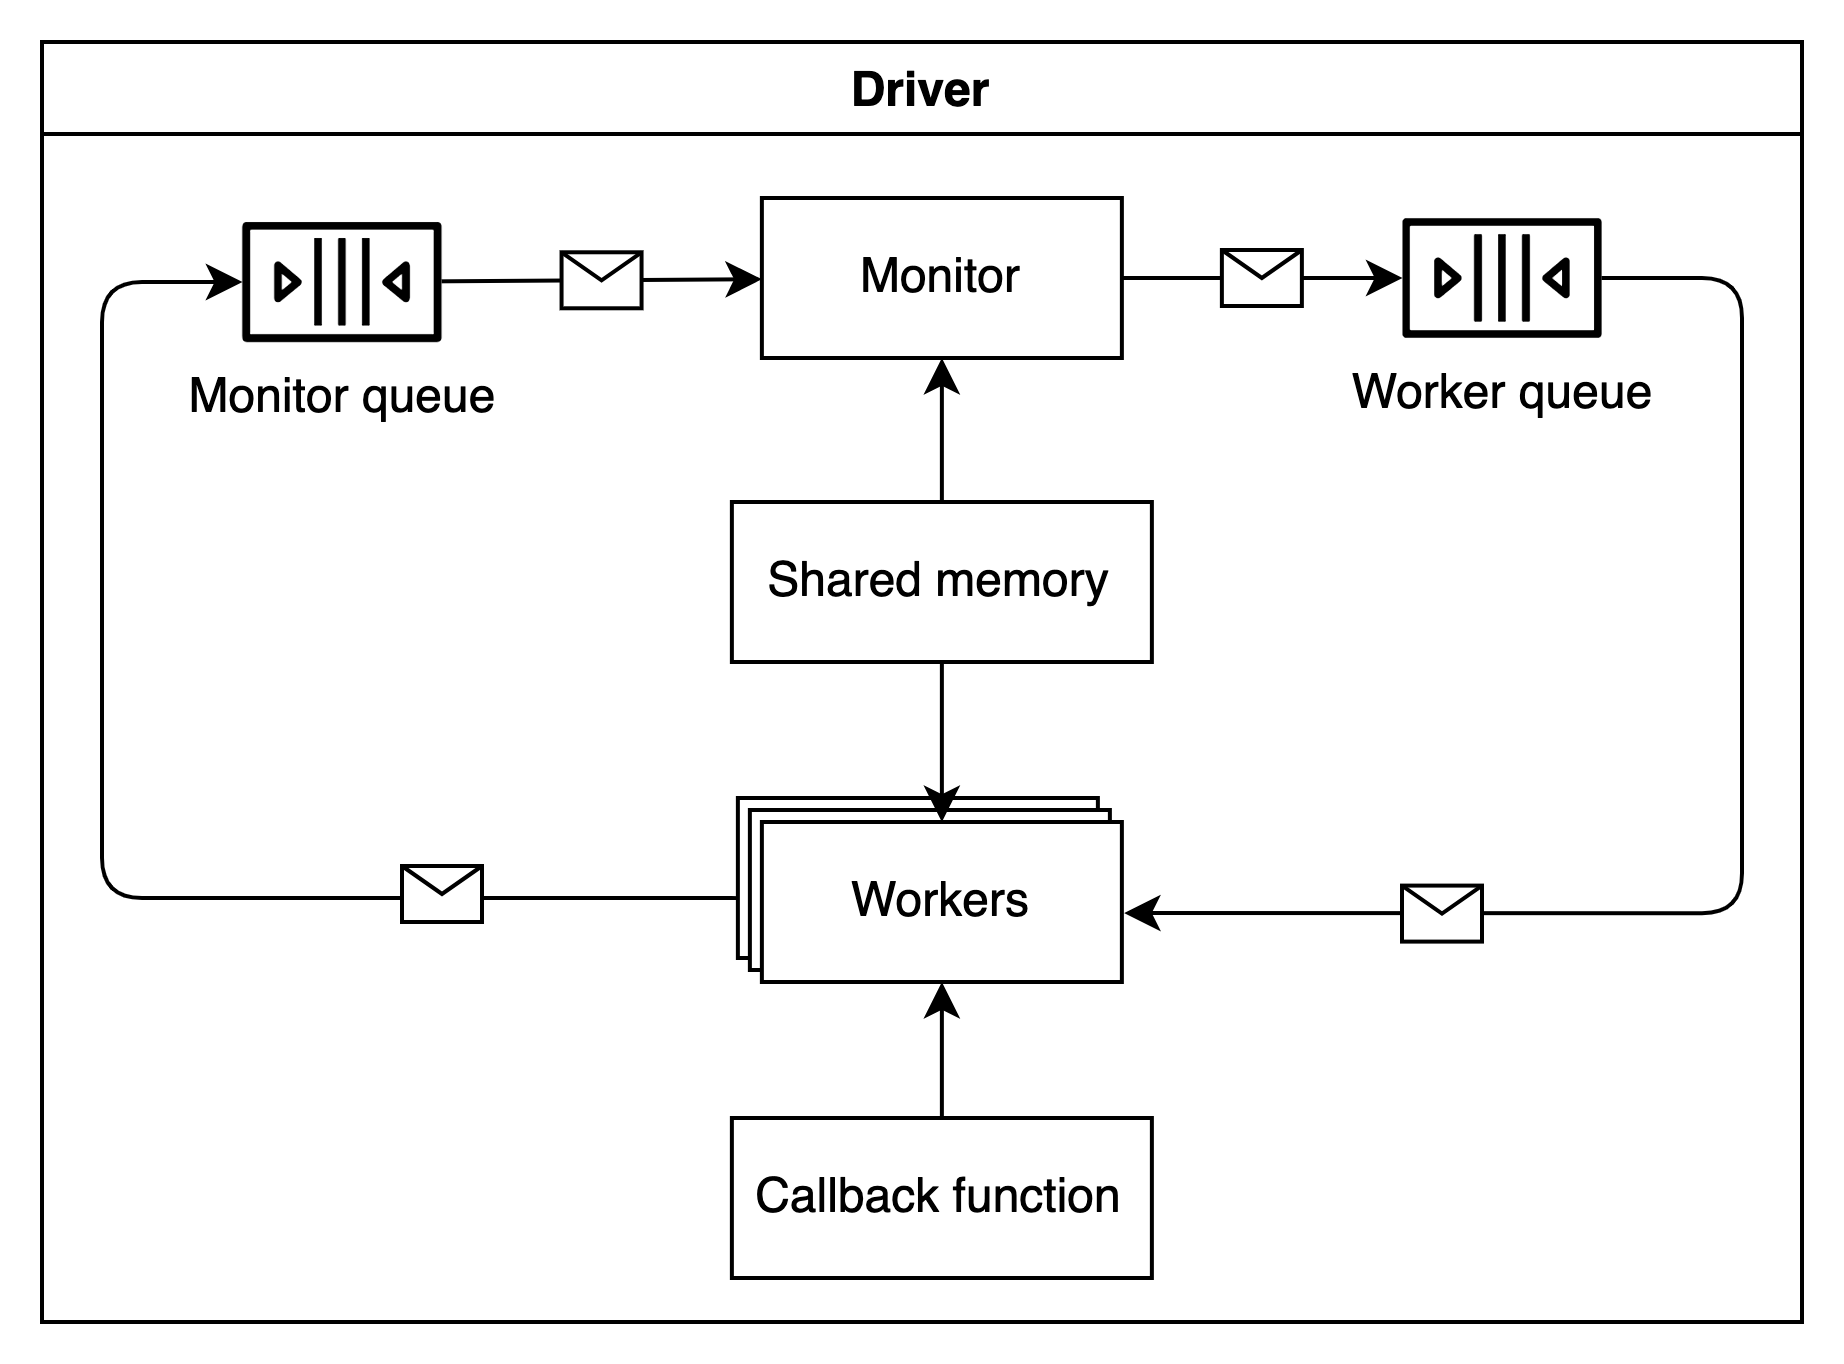
\includegraphics[width=\textwidth]{v3-architecture}
	\caption[Monitor-worker-driver framework]{Monitor-worker-driver framework.
		The \emph{monitor} is a stateful actor that is responsible for any mutable state of the program. A \emph{worker} (e.g., threads, processes, etc.) is a stateless entity that consumes monitor-produced messages from the \emph{worker queue}. Following the strategy design pattern \cite{Gamma1994}, worker behavior is defined by a \emph{callback function} which may use the attributes of a message to decide on how to process it. Any side effects of processing a message from the worker queue is encapsulated in a message and added to the \emph{monitor queue}. The monitor then consumes messages from the monitor queue, updates the state of the program, and produces messages in response for the workers to consume. The use of queues follows the mediator design pattern \cite{Gamma1994} in that the monitor and workers communicate indirectly. Any immutable state of the program can be efficiently accessed by both the monitor and the workers in \emph{shared memory}. The \emph{driver} is responsible for initiating the monitor and workers, waiting for the monitor to terminate message-passing, and returning the program output.}
	\label{fig:v3-architecture}
\end{figure}

\begin{figure}[htbp]
\centering
\begin{lstlisting}[
caption={[Monitor-worker-driver framework code]Monitor-worker framework code. The \texttt{BaseMonitor} is responsible for observing the message-passing between workers and maintaining any state of the program. The \texttt{BaseDriver} defines the rest of the message-passing program by first completing any required setup, and then returning the result from the monitor. It is composed of a worker queue instance, a monitor queue instance, a worker callback function, and the number of workers to instantiate. The type variables \texttt{Q} and \texttt{M} are used to indicate the types of the queue and message, respectively. The \texttt{BaseMonitor.call(Q, Q)} method follows the template design pattern in that it specifies the composition of multiple abstract methods and leaves their implementation to subclasses \cite{Gamma1994}.},
label=listing:v3-code]
from abc from ABC
from typing import Any, TypeVar

Q, M = TypeVar("Q"), TypeVar("M")

class BaseMonitor(ABC):
    __slots__ = ()

    def call(self, mqueue: Q, wqueue: Q) -> Any:
        while not self.should_terminate():
            # Get a message from the monitor queue.
            msg = self.get(mqueue)
            # Only process the message if necessary.
            if self.should_process(msg):
                # Optionally modify the message.
                msg = self.transform(msg)
                # Update the state of the monitor.
                self.update(msg)
                # Put the message in the worker queue.
                self.put(wqueue, msg)

class BaseDriver(ABC):
    __slots__ = "monitor", "mqueue", "wqueue", "callback", "n_workers"

    def call(self, inputs: Any) -> Any:
        # Perform any necessary setup before starting.
        self.setup(inputs)
        return self.monitor.call(self.mqueue, self.wqueue)
	\end{lstlisting}
\end{figure}

\par For risk propagation, a \texttt{RiskMonitor} monitor was implemented. It terminates when any of the following conditions are satisifed. The default behavior is to terminate once the monitor queue is empty.

\begin{itemize}
	\item The monitor has received \texttt{max\_msgs} messages.
	\item A duration of \texttt{max\_duration} has elapsed.
	\item No variable vertex has updated after \texttt{n\_msgs\_early\_stop} messages.
	\item No messages have been received \texttt{n\_retries} times after \texttt{timeout} time.
\end{itemize}

\par Only messages that are likely to induce an update to the state of the monitor are processed. The \texttt{send\_threshold} parameter allows us to vary the strictness of this likelihood. For a message sent by a variable node, the monitor only allows it if the value, scaled by \texttt{send\_threshold}, is greater than the current value of the variable vertex. This does not guarantee that it will invoke an update after the receiving factor vertex processes it, but it does prevent messages that would obviously not cause a variable vertex to update its value. Similarly, for a factor message, the monitor only allows it if the value, scaled by \texttt{send\_threshold}, is greater than the current value of the receiving variable vertex. Unlike variable messages, this guarantees against sending ineffective messages. Even if no other terminating condition is specified, the nature of \texttt{filter(M)} will gradually cause message passing to terminate. No transformation is applied to messages. The \texttt{update(M)} method contains the logic corresponding to the terminating conditions specified earlier. The monitor also updates the value of a variable vertex if the message value is greater than its current value.

\par The \texttt{RiskPropagation} driver exectutes risk propagation. Its \texttt{setup(Any)} method (1) creates the factor graph and stores it in shared memory, (2) sets the initial state of the monitor to be the maximum risk score of each variable vertex, and (3) adds all risk scores to the monitor queue. The \texttt{call(Any)} method (1) calls \texttt{setup(Any)}, (2) initializes \texttt{n\_workers} workers and the monitor, and (3) returns the state of the monitor, which is the exposure score of variable vertex.

\par Compared to the approach in Section \ref{sec:subgraph-actors}, this implementation provides a cleaner design and less communication overhead. However, what prompted me to consider (yet another) an alternative implementation was its scalability. As evidenced by Listing \ref{listing:v3-code}, the MWD framework is just a way of organizing an algorithm around the monitor while loop. Because the monitor processes messages serially, it is a bottleneck for algorithms in which the workers perform fine-grained tasks. Indeed, the Ray documentation notes that the parallelization of small tasks is an antipattern because the interprocess communication cost exceeds the benefit of multiprocessing [CITE]. Unfortunately, the functionality of a variable vertex and factor vertex is too fine-grained, so the scalability of the MWD framework is no better than a serial implementation.

% TODO
\section{Subgraph Actors with Projection}\label{sec:projected-subgraphs}

Improvements:
1. Best functioning implementation thus far 

Drawbacks:
1. Heavily dependent on the graph partitioning

% TODO
\section{Thinking Like a Vertex with Actors}\label{sec:vertex-actors}

Improvements:
1. Distributed; a drawback of all but the first approach
2. Decentralized; a drawback of all previous approaches
3. Robust; allows for delays in the changes of the contact graph with caching
4. Scalable and performant

Drawbacks:
1. Concurrent execution is difficult to reason about